\section{Desktop - Simulador da Linha (item 2a)}

\subsection{Função}

O Desktop (\cod{simulador/main.py}, iniciado por \cod{run\_mock.ps1}) é um aplicativo PyQt6 que substitui o CLP e o Gateway quando o hardware não está disponível, falando os mesmos protocolos: envia cada Andon pelo protocolo binário de 16 bytes ao receptor (TCP 15000) e publica a telemetria no mesmo servidor OPC UA seguro, com os mesmos 72 NodeIds do Gateway. Dessa forma, o receptor e a Dashboard funcionam sem alteração com o simulador ou com a linha real. A janela (Figura \ref{fig:desk1}) mostra, para os postos 01 a 12, os quatro Andons (Qualidade, Equipamento, Processo e Material) e os campos de Takt time e último ciclo; o rodapé informa o estado do TCP e a fila (pendentes e confirmados), e o cabeçalho, o estado do OPC UA.

\begin{figure}[H]
    \centering
    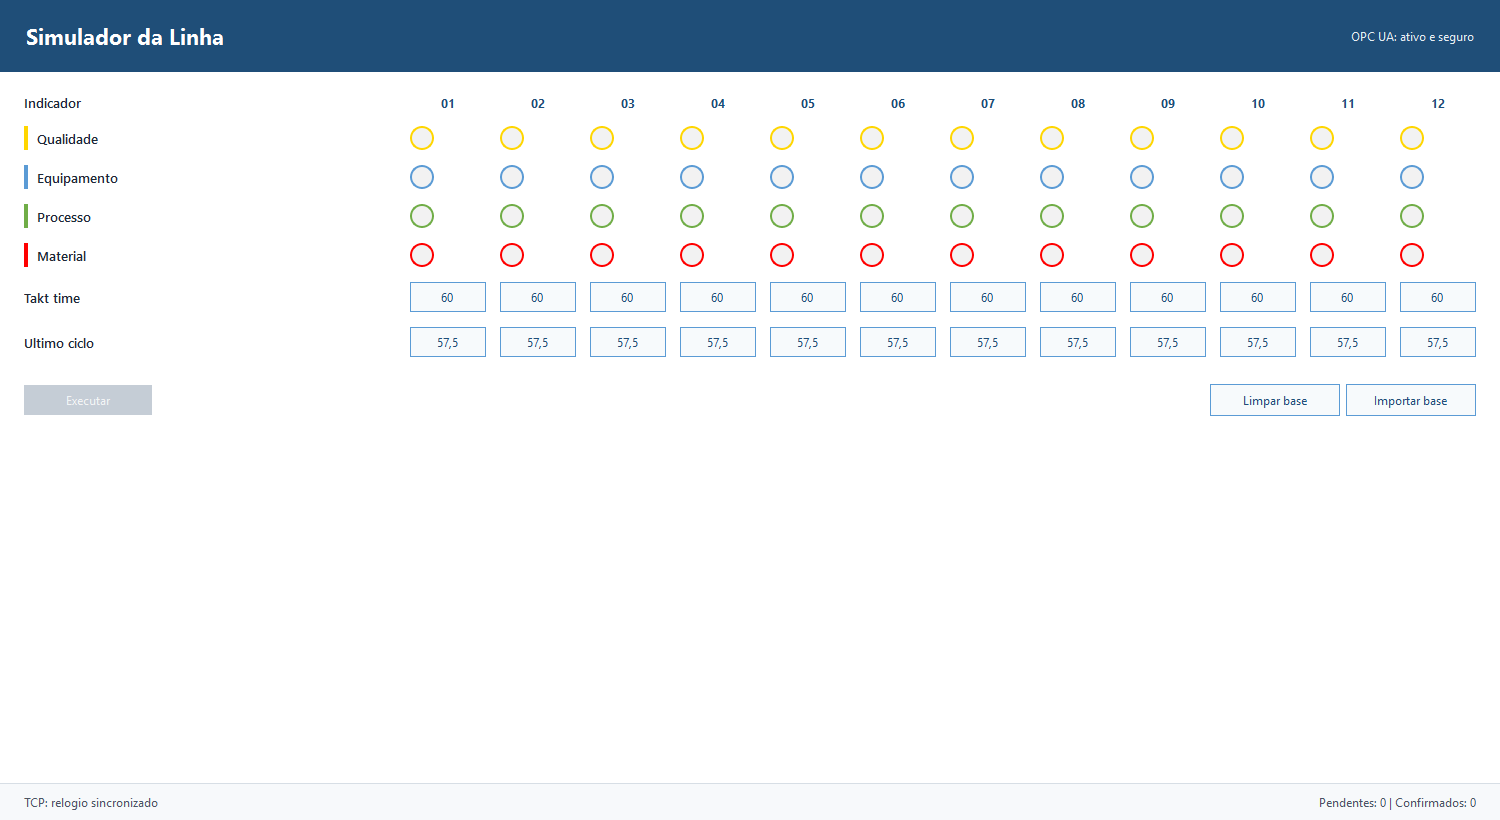
\includegraphics[width=1.00\textwidth]{Imagens/desk_01_inicial.png}
    \caption{Janela do Simulador da Linha ao iniciar: 48 Andons desligados, Takt 60 s e último ciclo 57,5 s (valores de \cod{config.toml}), OPC UA ``ativo e seguro''. (arquivo: Imagens/desk\_01\_inicial.png)}
    \label{fig:desk1}
\end{figure}

\subsection{Regras de funcionamento}

\begin{itemize}
    \item Um clique registra uma única data e hora lógica, alterna somente o botão escolhido e, na mesma transação SQLite, grava o novo estado e o pacote imutável de 16 bytes. A interface só muda depois do COMMIT; se o banco falhar, o estado visual não muda e uma mensagem de erro é exibida.
    \item A fila de saída é global e estritamente FIFO pelo identificador autoincremental. Apenas um evento fica em trânsito; o seguinte espera o ACK válido do anterior. Falhas usam esperas de 1, 2, 5, 10 e 30 s, permanecendo em 30 s; ao reiniciar, os estados são restaurados e o primeiro evento pendente é retomado.
    \item As quatro categorias de um posto são independentes e podem ficar ligadas ao mesmo tempo (\cod{test\_multiple\_categories\_can\_be\_on}); cada mudança gera um evento próprio.
    \item Takt time e último ciclo podem ser editados por posto e são publicados no OPC UA pelo botão \textbf{Executar}. \textbf{Importar base} reproduz planilhas \cod{.xlsx}, \cod{.xlsm} ou \cod{.csv} publicando um par Takt/ciclo por segundo; 26 planilhas de exemplo estão em \cod{bases\_exemplo/} (operação estável, gargalo fixo no P06, gargalo migrando, linha balanceada e desbalanceada, entre outras).
    \item Com \cod{sync\_on\_start = true}, o Desktop pede a hora ao receptor (pacote \cod{00 01} seguido de 14 bytes zero) e passa a usar um relógio lógico monotônico, sem alterar o relógio do Windows.
\end{itemize}

\subsection{Evidência: Desktop $\rightarrow$ receptor $\rightarrow$ Dashboard}

Em 21/11/2026 o Desktop foi executado com um receptor dedicado (portas 4851, 8092 e 15011). Na partida, o Desktop sincronizou o relógio (\cod{HORA respondida} às 20:24:45) e o cliente OPC UA do receptor conectou-se ao servidor do simulador. Foi acionado o Andon de Material do P03 e, 18 s depois, liberado (Figuras \ref{fig:desk2} e \ref{fig:desk3}). O terminal do receptor registrou:

{\scriptsize
\begin{verbatim}
[2026-11-21T20:24:51.208851-04:00] posto=03 botao=Material estado=ON resultado=ON ACK=enviado
[2026-11-21T20:25:09.694850-04:00] posto=03 botao=Material estado=OFF resultado=OFF ACK=enviado
\end{verbatim}
}

O banco do Desktop (\cod{outbox\_event}) registra os dois pacotes, \cod{00 01 00 03 11 26 20 21 50 24 20 06 00 04 00 01} (ON) e \cod{... 00 04 00 02} (OFF), ambos com \cod{delivery\_status = confirmed}, \cod{attempts = 0} e 11,5 ms e 10,5 ms entre a gravação na fila e o ACK do receptor. Na base histórica do simulador (\cod{simulador/data/mock\_line.db}) os quatro eventos gerados em 21/11/2026 entre 20:01 e 20:02 foram confirmados entre 10,5 e 14,5 ms.

\begin{figure}[H]
    \centering
    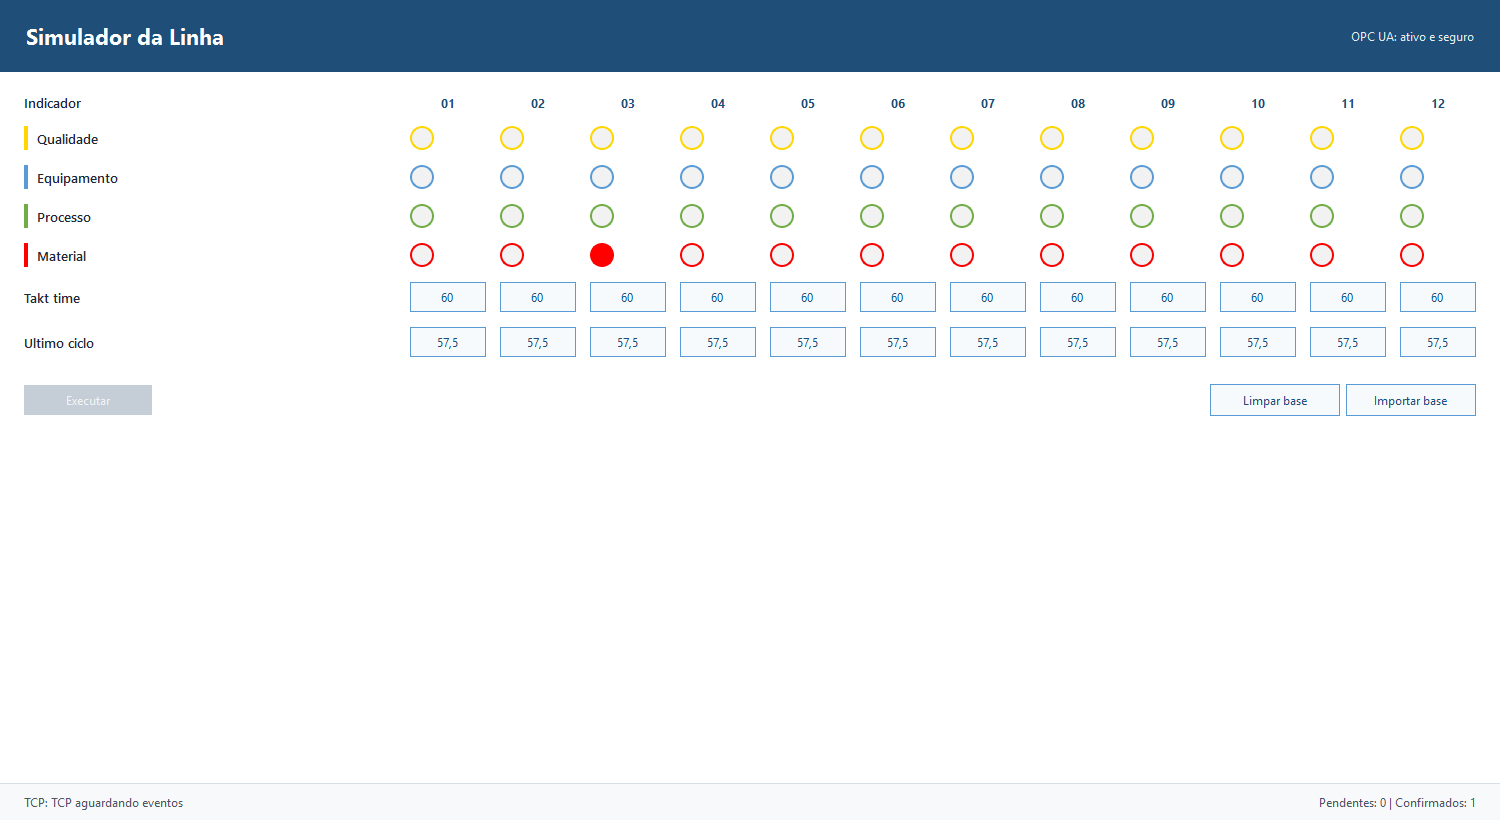
\includegraphics[width=1.00\textwidth]{Imagens/desk_02_andon_ativo.png}
    \caption{Andon de Material do posto 03 aceso; rodapé ``Pendentes: 0 | Confirmados: 1'' (o evento ON já recebeu o ACK). (arquivo: Imagens/desk\_02\_andon\_ativo.png)}
    \label{fig:desk2}
\end{figure}

\begin{figure}[H]
    \centering
    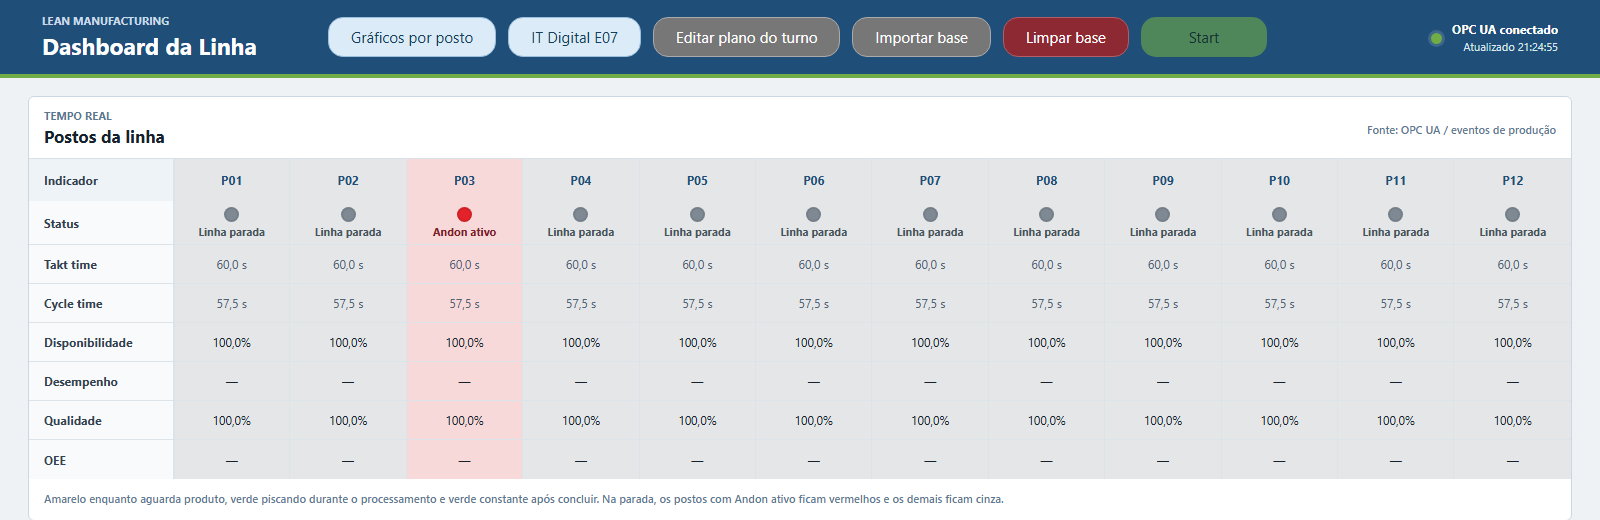
\includegraphics[width=1.00\textwidth]{Imagens/desk_04_dashboard_simulador.png}
    \caption{Dashboard alimentada pelo Desktop no mesmo instante: coluna P03 em vermelho (``Andon ativo'') e os demais postos em ``Linha parada''. (arquivo: Imagens/desk\_04\_dashboard\_simulador.png)}
    \label{fig:desk3}
\end{figure}

Os testes automatizados do Desktop (Tabela \ref{tab:testes}, seção 9) cobrem a atomicidade do clique (\cod{test\_toggle\_is\_atomic\_and\_persists\_queue}), o \textit{rollback} em falha de codificação, a restauração após reinício, a fila FIFO com reenvio (\cod{test\_sender\_retries\_head\_then\_preserves\_fifo}), a janela com 12 postos e a publicação da planilha importada com intervalo de 1 s.
